\documentclass[conf]{new-aiaa}
%\documentclass[journal]{new-aiaa} for journal papers
\usepackage[utf8]{inputenc}

\usepackage{graphicx}
\usepackage{amsmath}
\usepackage[version=4]{mhchem}
\usepackage{siunitx}
\usepackage{longtable,tabularx}
\usepackage{footnote}
\usepackage{mhchem}
\usepackage{physics}
\usepackage{array,makecell,booktabs}
\newcolumntype{M}[1]{>{\centering\arraybackslash}m{#1}}
\usepackage[super]{nth}
\makesavenoteenv{tabular}
\setlength\LTleft{0pt}

\graphicspath{{figures/}}

\begin{document}

\section{Discussion}

This section presents estimates of the cost-per-flight of various reuse strategies. Two strategies, (downrange, rocket-propelled, propulsive landing, full recovery) and (downrange, no propulsion, parachute, full recovery), are shown to dominate the other strategies on cost. However, parachute recovery of the full first stage is likely only practical for small launch vehicles\footnote{A small stage on parachutes could be recovered in midair or on a ship, or survive landing on land. A large stage on parachutes may need to land directly in the ocean, which would increase recovery and refurbishment expenses.}, and it will also be shown that first stage reuse is not favorable for small launch vehicles. Thus, downrange propulsive landing appears to be the dominant strategy.

Launch rate is also a critical factor in the economics of reuse. Increasing launch rate further reduces cost-per-flight, and also allows the investment in reuse development to be paid off more quickly. Efficient first stage reuse may allow for an increase in launch rate. A market that can support a high (>20 flights/year) launch rate may be a critical factor for the economic viability of a first stage reuse.

The discussion is organized as follows: the first subsection shows the distribution of cost-per-flight estimates under a generic dispersion of the model input parameters. The subsequent subsections examine the effect of number of reuses, launch rate, and launch vehicle size on cost. Finally, the last section discusses whether the present value of cost savings from reuse is enough to justify the initial investment in its development.

\subsection{Strategy cost-per-flight estimates}

In order to evaluate the cost per flight distributions for various first stage reuse strategies, we again perform a Monte Carlo analysis. This is implemented by evaluating the performance and cost models in sequence, sampling from generic distributions of model input parameters. For a given payload, we first evaluate the required masses of the launch vehicle elements for different reuse strategies using the performance model. Then, those resulting masses are used with the cost model to evaluate the cost per flight of the launch vehicles for each reuse strategy. Some of these cost per flight distributions are shown in Figures \ref{fig:strategy_cost_LEO_kerosene_pld10000}- \ref{fig:strategy_cost_LEO_H2_pld10000}. 

\begin{figure}[hbt!]
    \centering
    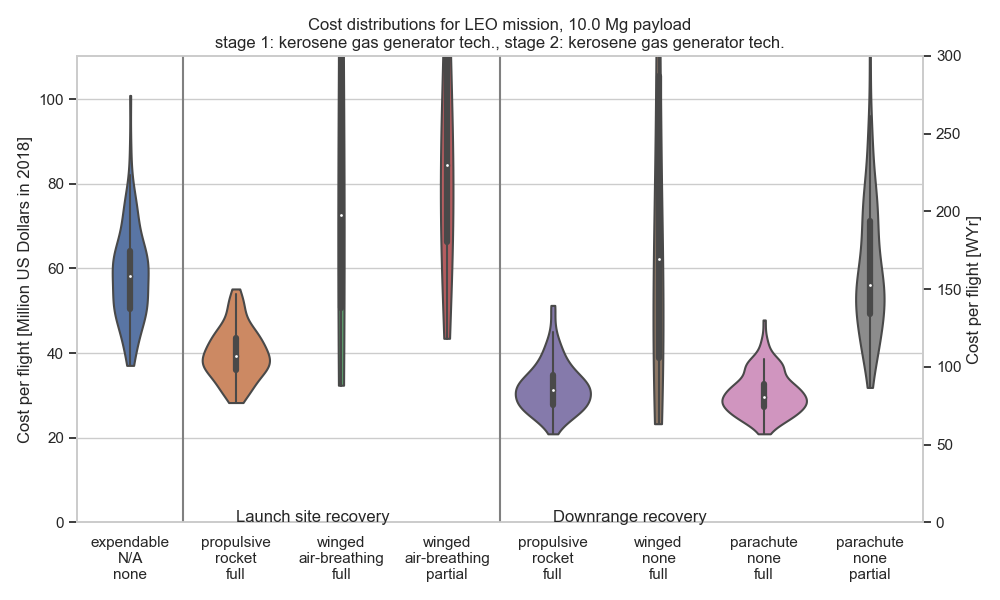
\includegraphics[width=\textwidth]{../../lvreuse/analysis/combined/plots/strategy_cost_LEO_kerosene_pld10000}
    \caption{\label{fig:strategy_cost_LEO_kerosene_pld10000} TODO caption.}
\end{figure}

\begin{figure}[hbt!]
    \centering
    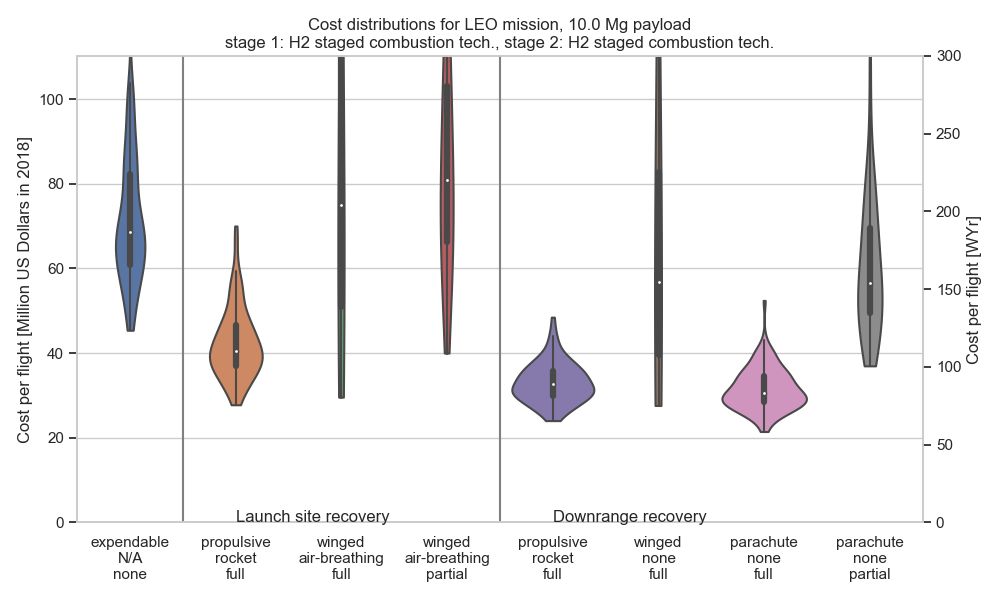
\includegraphics[width=\textwidth]{../../lvreuse/analysis/combined/plots/strategy_cost_LEO_H2_pld10000}
    \caption{\label{fig:strategy_cost_LEO_H2_pld10000} TODO caption.}
\end{figure}

The downrange propulsive landing and parachute strategies for full first stage recovery show very similar distributions with the lowest cost per flight distributions among all the strategies. However, as mentioned previously, parachute recovery of the full first stage is not very feasible for large vehicles. Therefore downrange propulsive landing is the most effective strategy for achieving the lowest cost per flight. 

We see broad distributions for winged recovery strategies due to a small number of historical reference projects available for fitting the production CER coefficients. This lack of data leads to large uncertainties in the coefficient values, resulting in large uncertainties in the output cost per flight distributions. 

It is also interesting to compare the cost per flight distributions for the two different technology choices (kerosene with gas generator and H2 with staged combustion). Despite the hydrogen technology choice yielding slightly better payload performance, the cost per flight distributions show slightly lower costs for kerosene. This result likely stems from two reasons:

\begin{itemize}
  \item The cost per kilogram of inert mass for producing a vehicle using hydrogen propellant is greater than that for kerosene. 
  \item The inert mass of a vehicle using hydrogen propellant is generally greater than that of kerosene for a given payload mass.
\end{itemize}

Additionally, partial reuse strategies do not seem to yield any significant cost per flight savings. For these reuse strategies, the extra mass required to make a first stage vehicle partially recoverable does not make up for any cost savings achieved by reusing the high-value components. 

% Maybe include some GTO stuff here if there is room.

\subsection{Effect of number of reuses and launch rate on cost per flight}
stack plot with reuse sweep- show why cost declines with number of reuses
cpf vs. reuse plot with varying launch rate curves - shows significant decrease in cost with increasing launch rate for low launch rates
cpf vs. reuse plot for different strategies 

In order to look at the breakdown of costs for a launch vehicle with a reusable first stage, we consider a point cost estimate to demonstrate general trends. The following example evaluates a two stage launch vehicle carrying a 10,000 kg payload to LEO using kerosene and liquid oxygen propellants at a launch rate of 15 launches per year. We consider the case of a propulsive downrange landing to recover and reuse the entire first stage. The cost per flight is determined over a range of number of first stage uses. The results of this analysis are shown in Figure \ref{fig:cpf_stackplot_reuses_sweep}.

\begin{figure}[hbt!]
    \centering
    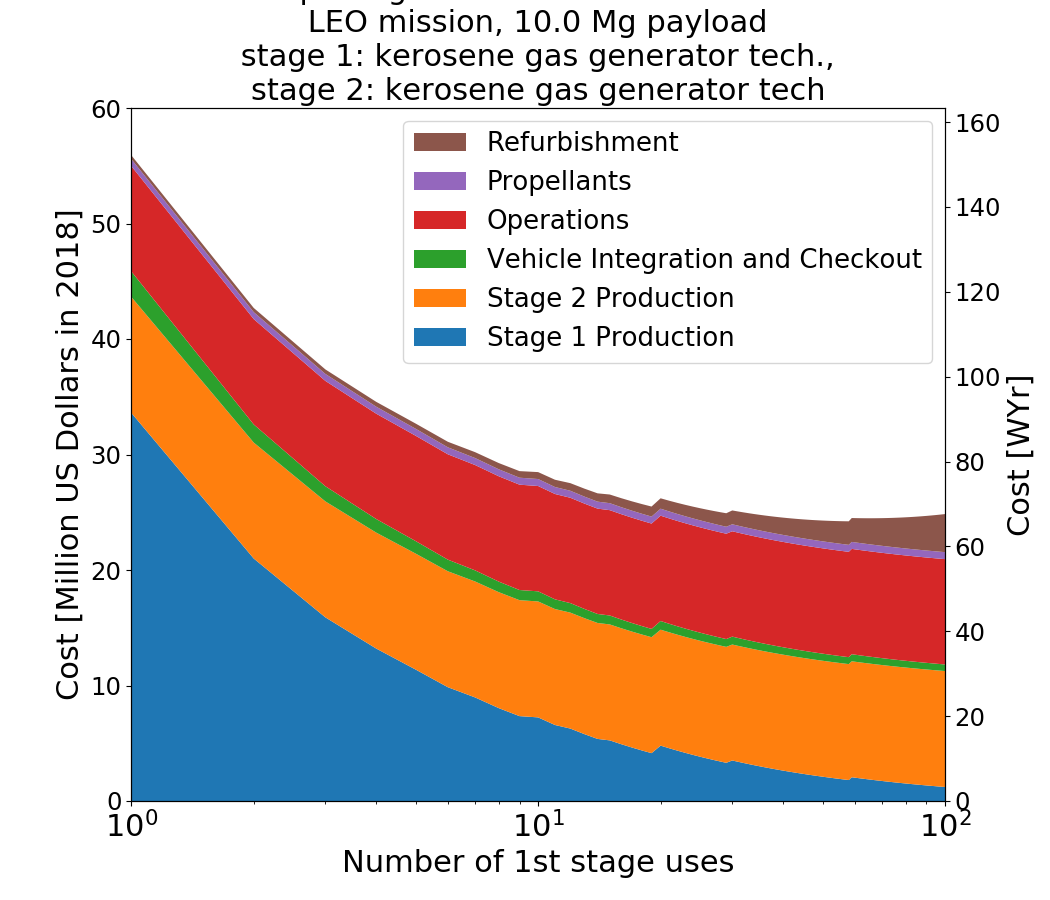
\includegraphics[width=\textwidth]{../../lvreuse/analysis/combined/plots/cpf_stackplot_reuses_sweep}
    \caption{\label{fig:cpf_stackplot_reuses_sweep} TODO caption.}
\end{figure}

Several things should be noticed from the results in Figure \ref{fig:cpf_stackplot_reuses_sweep}. First, the stage one productions costs per flight decrease dramatically as we increase the number of first stage reuses. This result is very intuitive -- as the cost of first stage production is spread over a larger number of flights, the per flight amortization share of the first stage production cost decreases. This leads to a reduction in the cost per flight. However, this trend of decreasing amortization share of first stage production costs is opposed by the refurbishment cost trends. As the number of first stage uses increases, the refurbishment cost per flight also increases. This is due to the fact that more components on the first stage will need inspected or replaced  as the number of reuses increases. 

These opposing trends lead to an interesting result: the total cost per flight trend achieves a minimum value. In the example in Figure \ref{fig:cpf_stackplot_reuses_sweep}, we see a minimum cost per flight around 57 first stage uses. After 57 uses of the first stage, it would be more cost effective to use a new first stage than to continue refurbishing the old one. It should be noted however that the number or reuses that will yield the minimum cost per flight is highly dependent on the refurbishment costs per flight. Higher or lower refurbishment costs per flight would lead to a different optimal number of first stage reuses.

The cost per flight is also affected by the annual launch rate. Most cost components in the cost per flight breakdown do not vary with launch rate, with the exception of the operations costs which are very sensitive to launch rate. The operations costs are heavily dependent on the number of employees required to operate a launch. For low launch rates, operations employees will be idle for a large portion of their time. This drives up the operations cost per flight since these employees must be retained despite low launch rates and idle time. The cost per flight trends with varied launch rates are given in Figure \ref{fig:cpf_reuses_sweep_vary_launch_rate}. 

\begin{figure}[hbt!]
    \centering
    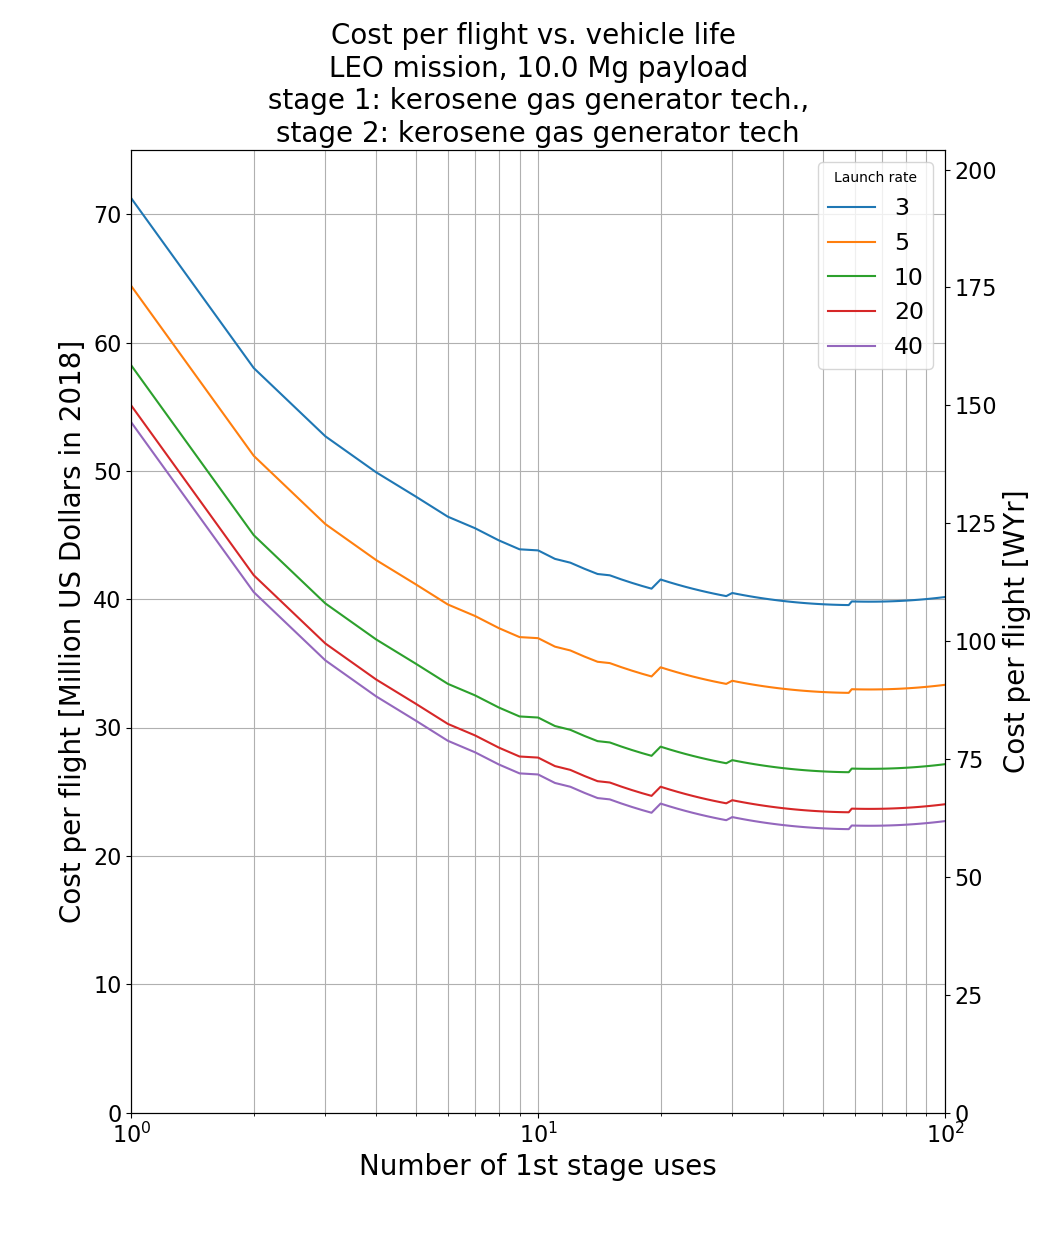
\includegraphics[width=\textwidth]{../../lvreuse/analysis/combined/plots/cpf_reuses_sweep_vary_launch_rate}
    \caption{\label{fig:cpf_reuses_sweep_vary_launch_rate} TODO caption.}
\end{figure}

As expected, Figure \ref{fig:cpf_reuses_sweep_vary_launch_rate} shows that the cost per flight is higher at lower launch rates, regardless of the number of first stage reuses. For low launch rates, we see a substantial decrease in the cost per flight for only a modest increase in launch rate. However, for high launch rates, further increases in launch rate do not have a large effect on the cost per flight. For instance, we see a large difference in cost per flight by increasing the launch rate from 3 to 5 launches per year. However, increasing the launch rate from 20 to 40 launches per year yields only very minimal cost per flight reductions. 

Now that we've established the general trends of the cost per flight with launch rate and number of first stage uses, we consider these trends for varying first stage reuse strategies. Figure \ref{fig:num_reuse_sweep_LEO_kerosene} shows the cost per flight trends for selected strategies over a range of number of first stage uses. We consider two cases in this analysis: 

\begin{itemize}
  \item First stage reuse has no effect on the vehicle launch rate. The first stage production rate is not the rate-limiting step of the launch rate. In this case, operations or second stage production are likely rate-limiting.
  \item First stage reuse increases the launch rate. The first stage production is the rate-limiting step for the vehicle launch rate. Increasing the vehicle first stage life increases the launch rate since first stages do not need to be produced as frequently.
\end{itemize}

\begin{figure}[hbt!]
    \centering
    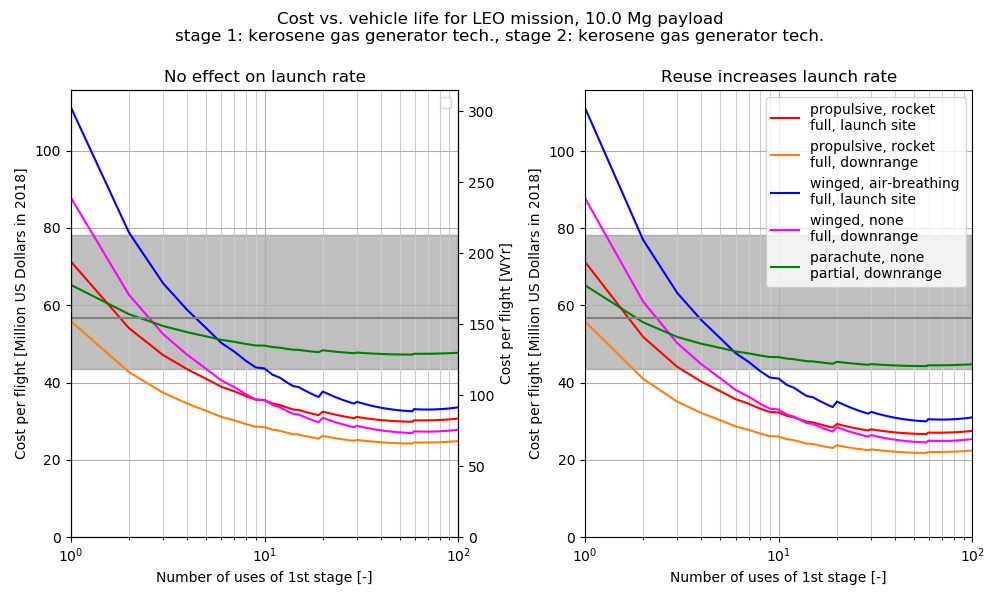
\includegraphics[width=\textwidth]{../../lvreuse/analysis/combined/plots/num_reuse_sweep_LEO_kerosene}
    \caption{\label{fig:num_reuse_sweep_LEO_kerosene} TODO caption.}
\end{figure}



\subsection{Effect of Launch Vehicle Size}
reuse doesn't make sense for smaller vehicles - costs not dominated by hardware cost

\subsection{Paying off development costs}

In our models and discussion so far, we have yet to consider the development costs of reuse strategies. 

\begin{figure}[hbt!]
    \centering
    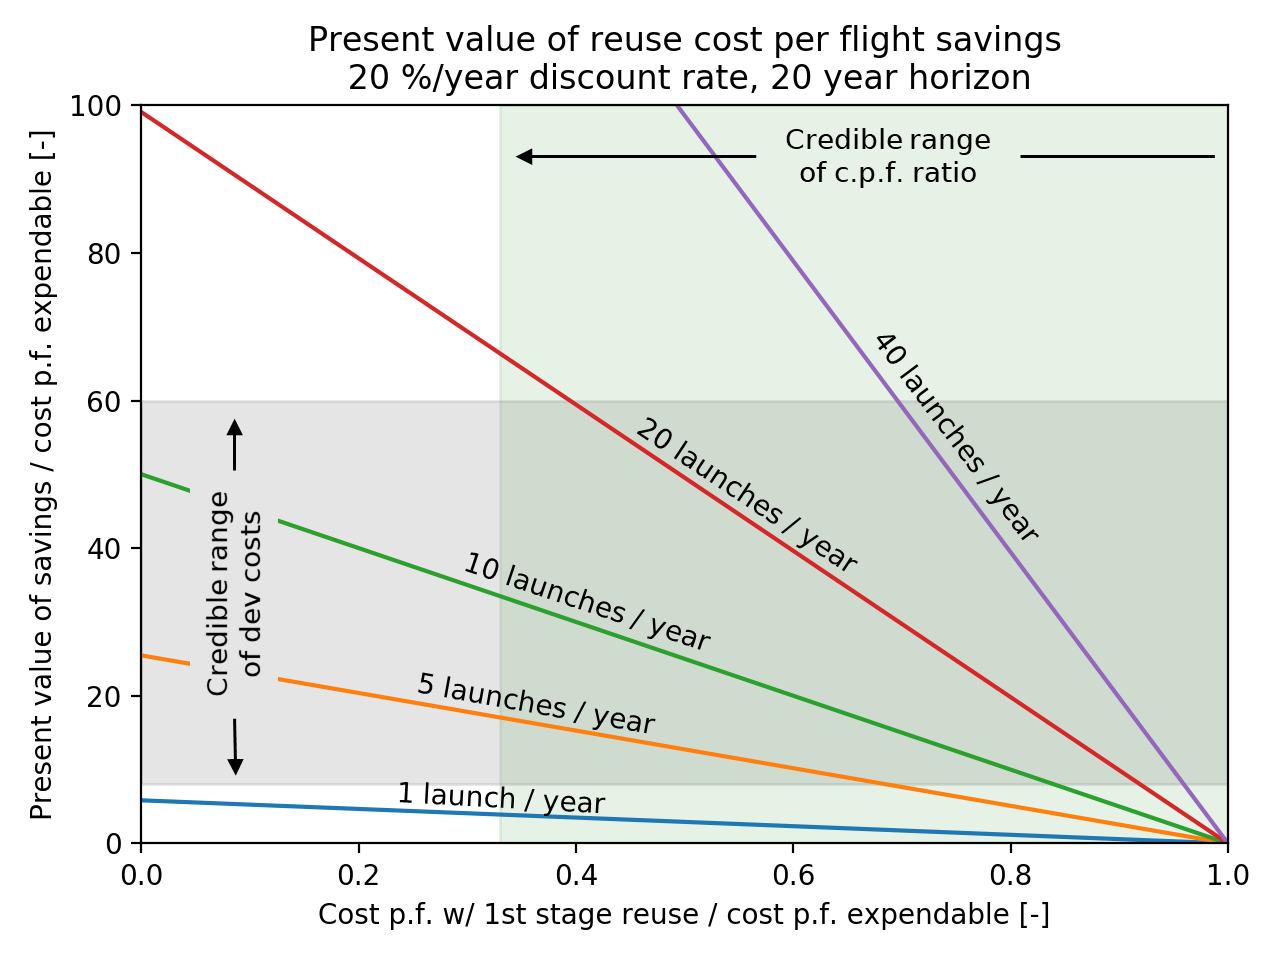
\includegraphics[width=\textwidth]{reuse_npv}
    \caption{\label{fig:reuse_npv} TODO caption.}
\end{figure}

\bibliography{first_stage_recovery}

\end{document}